\section{Theorie}
\label{sec:Theorie}
\subsection{Allgemein}
Wirken Kräfte auf einen Körper, so kann die Form und das Volumen des Körpers verändert werden.
Die Kräfte beziehen sich meist auf die Flächeneinheit und werden als Spannung $\sigma$ bezeichnet.
Die senkrecht zur Oberfläche wirkende Spannung wird als Normalspannung bezeichnet.
Tangential- oder Schubspannung heißt hingegen die parallel zur Oberfläche verlaufende Komponente.
Liegt bei der relativen Längenänderung $\frac{\Delta L}{L}$ ein linearer Zusammenhang vor, so beschreibt das Hook'sche Gesetz
\begin{equation}
    \sigma = E \cdot \frac{\Delta L}{L}
\end{equation}
die Deformation.
Dabei beschreibt $E$ der Elastizitätsmodul, $L$ die Länge und $\Delta L$ die Längenänderung des Körpers (siehe Abb. \ref{fig:spannung}).
Der Elastizitätsmodul ist eine materialabhängige Konstante des Werkstoffes.
Die Längenänderung $\Delta L$ kann nur mit genauen Messaperaturen direkt bestimmt werden.\\
Eine weitere Möglichkeit zur Bestimmung des Elastizitätsmodul ist die Biegung.
Hier genügt eine relativ kleine Kraft am Ende des Stabes um eine messbare Längenänderung zu bewirken.
\begin{figure}
    \centering
    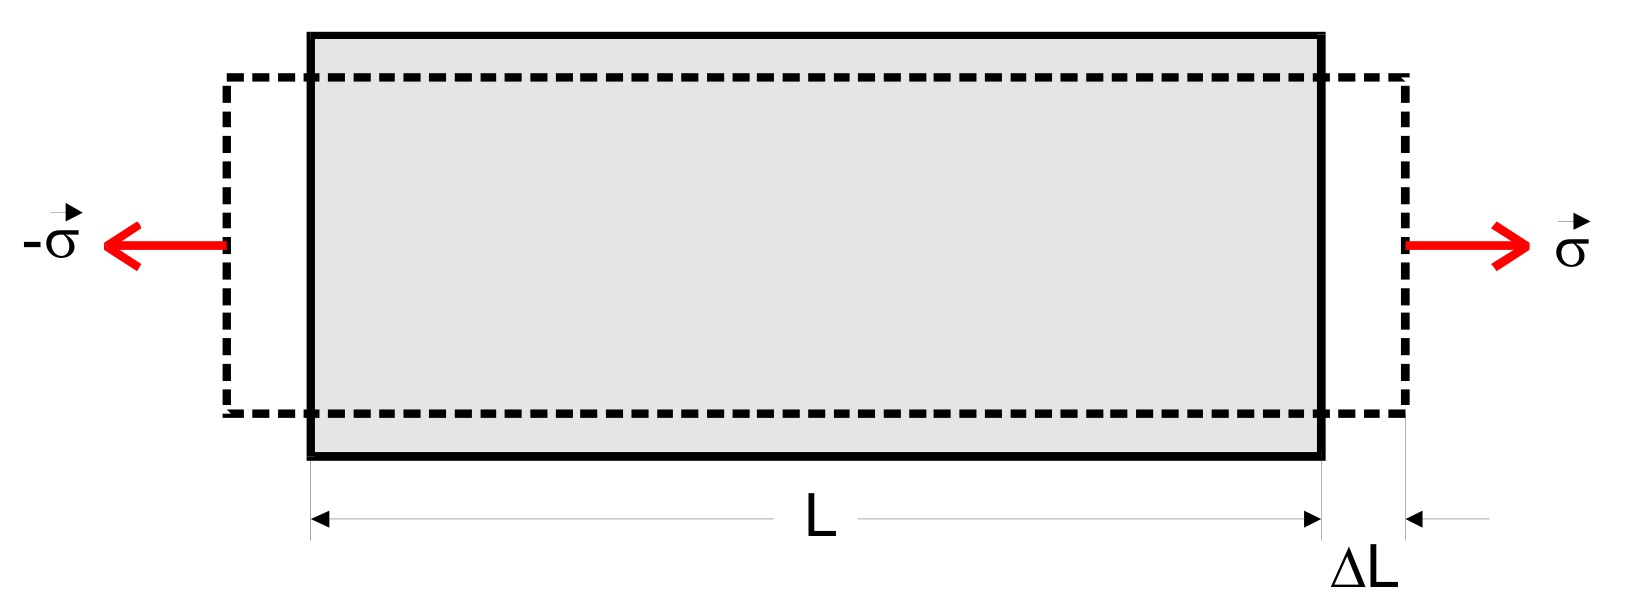
\includegraphics[width=0.75\textwidth]{content/data/spannung.jpg}
    \caption{Dehnung eines Stabes bei wirkender Normalspannung.\cite{anleitung}}
    \label{fig:spannung}
\end{figure}
\subsection{Biegung - Einseitige Einspannung}
Ein homogener Stab wird auf einer Seite eingespannt und am anderen Ende wirkt eine Kraft $F$.
Es wird die Durchbiegung $D(x)$ gemessen.
Sie beschreibt die Verschiebung von einem Oberflächenpunkt bei einer Biegung (siehe Abb. \ref{fig:stab_einseitig}).
Mithilfe von $x$ und $D(x)$ kann die Materialkonstante bestimmt werden.
\begin{figure}
    \centering
    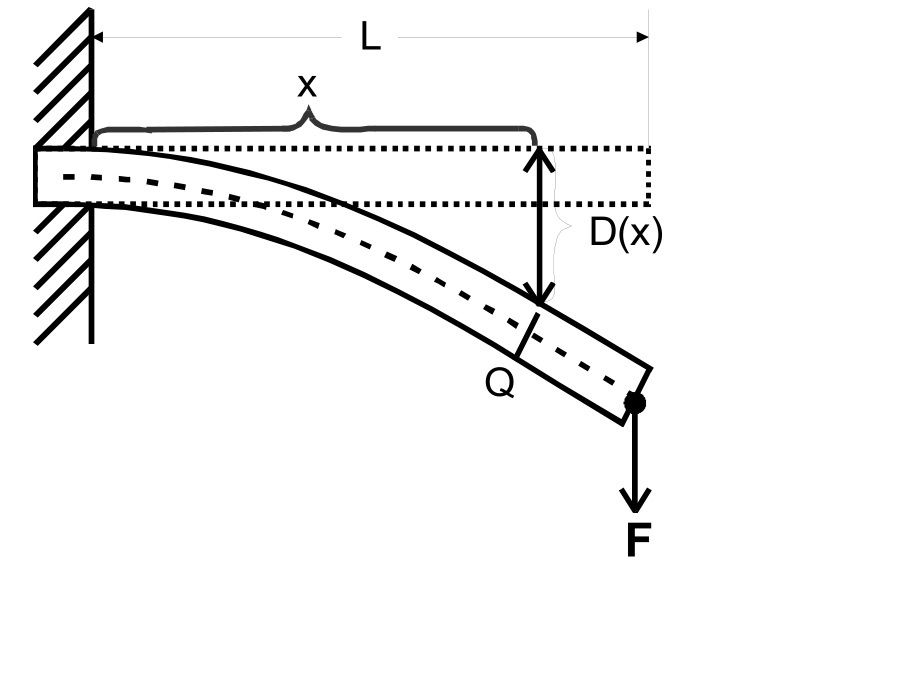
\includegraphics[width=0.5\textwidth]{content/data/biegen_einseitig.jpg}
    \caption{Stange mit Querschnitt $Q$ wird durch eine äußere Kraft $F$ einseitig gebogen.\cite{anleitung}}
    \label{fig:stab_einseitig}
\end{figure}
Die Kraft $F$ wirkt senkrecht auf den Querschnitt $Q$ des Stabes.
Sie bewirkt ein bestimmtes Drehmoment $M$ in Abstand $x$, das den Stab verbiegt.
Dabei werden obere Schichten gedehnt und die unteren gestaucht.
Durch die Elastizität des Materials stellt sich ein Gleichgewichtszustand und eine Durchbiegung $D$ ein.
In den oberen Schichten treten Zugspannungen auf, in den uneteren Schichten Druckspannungen und dazwischen befindet sich ein Gebiet ohne Spannung.
Dieses Gebiet wird als neutrale Faser bezeichnet.
Das Drehmoment $M_\sigma$ berechnet sich nach
\begin{equation}
    M_\sigma = \int_Q y \sigma(y) \symup{d}q
\end{equation}
mit dem Abstand $y$ des Flächenelements $\symup{d}q$ zur neutralen Faser $x$ (siehe Abb. \ref{fig:drehmoment}).
\begin{figure}
    \centering
    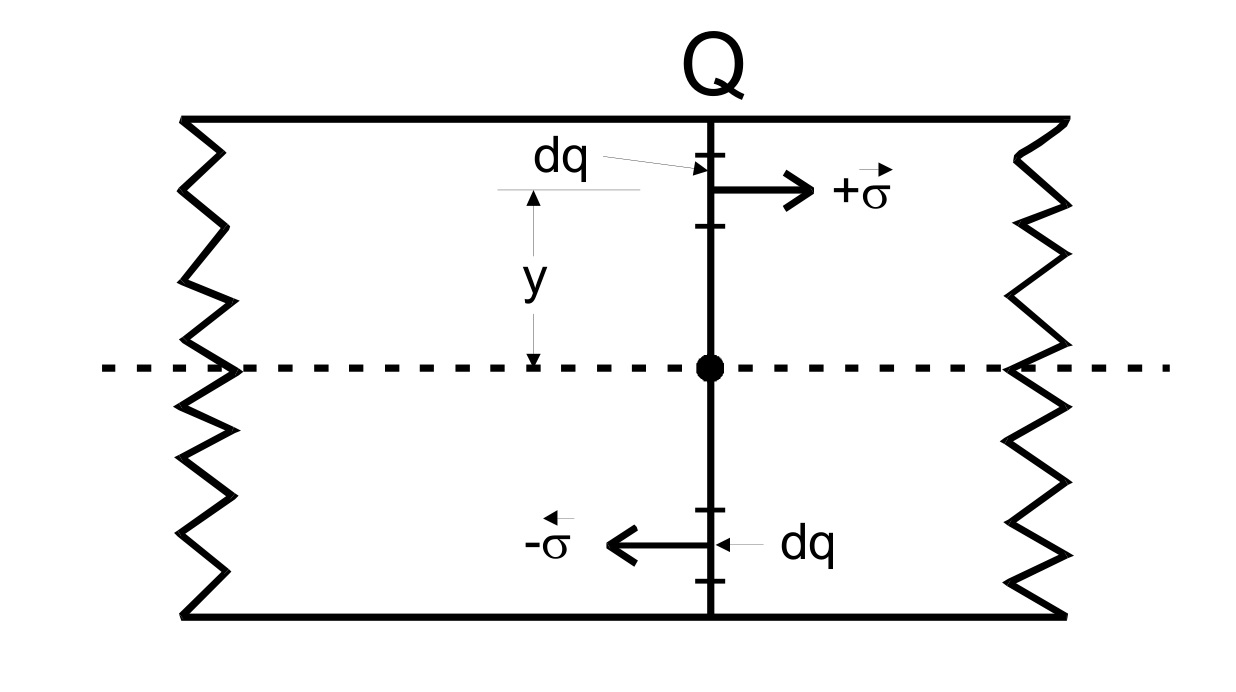
\includegraphics[width=0.5\textwidth]{content/data/drehmoment.jpg}
    \caption{Stange zur Veranschaulichung des Trägheitsmoment.\cite{anleitung}}
    \label{fig:drehmoment}
\end{figure}
Nach einer bestimmten Zeit stellt sich ein Gleichgewicht
\begin{equation}
    M_\text{F} = M_\sigma
    \label{eqn:einseitig1}
\end{equation}
ein.
Außerdem gilt die Beziehung
\begin{equation}
    \sigma = E \frac{\delta x}{\Delta x}
    \label{eqn:einseitig2}
\end{equation}
und
\begin{equation}
    \delta x = y \Delta \varphi = y \frac{\Delta x}{R} .
    \label{eqn:einseitig3}
\end{equation}
Hierbei steht $R$ für den Krümmungsradius der Faser an der Stelle $x$.
Aus den Gleichungen \eqref{eqn:einseitig1} und \eqref{eqn:einseitig2} folgt
\begin{equation}
    \sigma(y) = E \frac{y}{R} .
    \label{eqn:einseitig4}
\end{equation}
Für geringe Kurvenkrümmungen kann die Näherung $\frac{1}{R} \approx \frac{\symup{d^2}D}{\symup{d}x^2}$ aus der Differentialgeometrie verwendet werden.
Mithilfe der Näherung ergibt sich für die Formel \eqref{eqn:einseitig4}
\begin{equation}
\sigma(y) = E y \frac{\symup{d^2}D}{\symup{d}x^2}
\end{equation}
und für die Momentengleichung \eqref{eqn:einseitig1}
\begin{equation}
    E \frac{\symup{d^2}D}{\symup{d}x^2} \int_Q y^2 \symup{d}q = F(L-x).
    \label{eqn:moment}
\end{equation}
Wird das Flächenträgheitsmoment
\begin{equation*}
    I := \int_Q y^2 \symup{d}q(y)
\end{equation*}
verwendet, so lässt sich die Gleichung \eqref{eqn:moment} durch Integration für $(0 \leq x \leq L)$ auf
\begin{equation}
    D(x) = \frac{F}{2EI} \left( Lx^2-\frac{x^3}{3} \right)
    \label{eqn:d_einseitig}
\end{equation}
vereinfachen.
\subsection{Biegung - Zweiseitige Auflage}
Der Stab wird an beide Enden aufgelegt und eine Kraft $F$ wirkt in der Mitte der Auflagepunkte (siehe Abb. \ref{fig:beidseitig}).
\begin{figure}
    \centering
    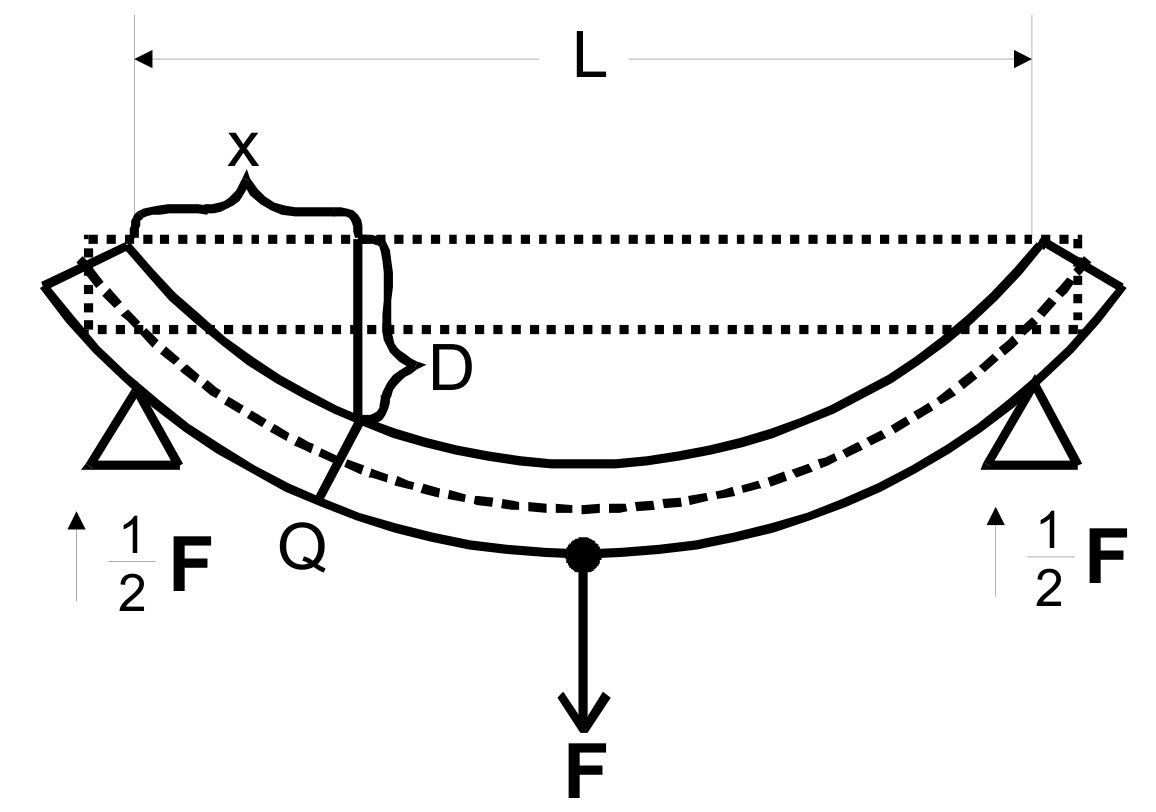
\includegraphics[width=0.5\textwidth]{content/data/beidseitig.jpg}
    \caption{Biegung eines Stabes mit zweiseitiger Auflage. \cite{anleitung}}
    \label{fig:beidseitig} 
\end{figure}
An der Querschnittsfläche $Q$ wirkt die Kraft $F/2$ mit dem Hebelarm $x$.
Im Bereich $0 \leq x \leq L$ folgt nach dem Drehmoment
\begin{equation*}
    M_\text{F} = -\frac{F}{2}x .
\end{equation*}
Das Drehmoment welches auf der andere Hälfte $\frac{L}{2} \leq x \leq L$ wirkt, berechnet sich nach
\begin{equation*}
    M_\text{F} = -\frac{F}{2}(L-x) .
\end{equation*}
Aus der Momentengleichung \eqref{eqn:moment} und Integration ergibt sich
\begin{equation}
    \frac{\symup{d}D}{\symup{d}x} = - \frac{x^2F}{4EI} + C \quad \text{für} \:\: 0 \leq x \leq \frac{L}{2}
    \label{eqn:mom1}
\end{equation}
und
\begin{equation}
    \frac{\symup{d}D(x)}{\symup{d}x} = -\frac{F}{2EI} \left( Lx-\frac{x^2}{2} \right) + C' \quad \text{für } \frac{L}{2} \leq x \leq L
    \label{eqn:mom2}
\end{equation}
für die jeweiligen Teilintervalle.
In der Mitte des Stabes besitzt die Biegekurve eine horizontale Tangente.
Daraus ergeben sich die Integrationskonstanten
\begin{equation}
    C = \frac{L^2F}{16EI}
    \label{eqn:konst1}
\end{equation}
und
\begin{equation}
    C' = \frac{3L^2F}{16EI} .
    \label{eqn:konst2}
\end{equation}
Mit den Konstanten \eqref{eqn:konst1}, \eqref{eqn:konst2} und anschließender Integration von \eqref{eqn:mom1}, \eqref{eqn:mom2}, folgt die gesuchte Gleichung für einen elastisch gebogenen Stab
\begin{equation}
    D(x) = \frac{F}{48 E I} \left( 3L^2x -4x^3 \right) \quad \text{für } 0 \leq x \leq \frac{L}{2}
    \label{eqn:moment_links}
\end{equation}
und
\begin{equation}
    D(x) = \frac{F}{48EI} \left( 4x^3-12Lx^2+9L^2x-L^3 \right) \quad \text{für } \frac{L}{2} \leq x \leq L .
\end{equation}